\documentclass{article}
\usepackage{standalone}
\usepackage{import}
\usepackage{xcolor}

\usepackage{subfigure}

%\usepackage{standalone}
\usepackage{fancyhdr}


\usepackage{import}
\usepackage{caption}
\usepackage{amsfonts, amsmath, amsthm}
\usepackage{makecell}
\usepackage{lastpage}
\usepackage{moresize}



\hyphenpenalty=10000


\usepackage[utf8x]{inputenc}
\usepackage[T1]{fontenc}
\usepackage[english]{babel}
\usepackage{graphicx}
%\usepackage[languagenames,fixlanguage,english]{babelbib}
\usepackage[pdftex]{hyperref}
%\usepackage{txfonts}
%\usepackage{subcaption}
\usepackage[a4paper,top=3cm,bottom=2cm,left=3.5cm,right=3.5cm,marginparwidth=1.75cm]{geometry}
\usepackage{algorithm2e}
\usepackage{pdflscape}

\usepackage[e, gameslogo]{Template/gameshf}






\usepackage{tikz}
\usepackage{pgfplots}
\usepackage{circuitikz}
\usepackage{tabularx}
\usepackage{rotating}
\usepackage{caption} 
\captionsetup[table]{skip=10pt}

\usetikzlibrary{calc,positioning,shapes,decorations.pathreplacing}

\tikzset{
	short/.style={draw,rectangle,text height=3pt,text depth=13pt,
		text width=7pt,align=center,fill=gray!30},
	long/.style={short,text width=1.5cm},
	verylong/.style={short,text width=4.5cm}
}


%% User defined
\newcommand{\N}{\mathbb{N}}
\newcommand{\Z}{\mathbb{Z}}
\newcommand{\Q}{\mathbb{Q}}
\newcommand{\R}{\mathbb{R}}
\newcommand{\C}{\mathbb{C}}
\newcommand{\funcA}{\mathfrak{a}}
\newcommand{\funcB}{\mathfrak{b}}
\newcommand{\funcC}{\mathcal{C}}
\newcommand{\funcU}{\mathcal{U}}
\newcommand{\funcV}{\mathcal{V}}
\newcommand{\funcW}{\mathcal{W}}
\newcommand{\simgrad}{\sym\nabla}
\newcommand{\heps}{{h,\varepsilon}}
\newcommand{\epsh}{{\varepsilon(h)}}
\newcommand{\eps}{{\varepsilon}}
\newcommand{\twoscale}{{\,\overset{2}{\rightharpoonup}\,}}
\newcommand{\drtwoscale}{{\,\overset{dr-2}{\rightharpoonup}\,}}
\DeclareMathOperator{\sym}{sym}
\DeclareMathOperator{\dvg}{div}

\newcommand{\wye}{\mathbin{\tikz[x=1ex,y=1ex]{\draw[line width=.1ex] (0,0)--(30:1)--++(-30:1) (30:1)--++(0,1);}}}
\newcolumntype{Y}{>{\centering\arraybackslash}X}

%\newtheorem{exmp}{Example}[section]
%\newtheorem{note}{Note}
%\newtheorem{theorem}{Theorem}[section]
%\newtheorem{proposition}[theorem]{Proposition}
%\newtheorem{corollary}{Corollary}
%\newtheorem{definition}[theorem]{Definition}
%\newtheorem{lemma}{Lemma}[theorem]

\headheight 40pt              %% put this outside
\headsep 10pt                 %% put this outside


\graphicspath{{./Images/Crane/}{./Images/Electronics/}{./Images/}}

% Source: 
%https://tex.stackexchange.com/questions/117990/unicode-math-breaks-declaremathoperator
\AtBeginDocument{
	\let\div\relax
	\DeclareMathOperator{\div}{div}
}

\usepackage{enumitem}
\setlist[description]{style=unboxed}

%opening
\title{STEM games 2019}
\author{Mentori}

\title{STEM Games Engineering Arena}
\date{}

\begin{document}
	%\maketitle
	
	\thispagestyle{empty}
	\newpage
	\thispagestyle{empty}
	\vspace*{0cm}
	\begin{center}
		
		\textbf{\Huge{STEM Games 2019}}\\
		\vspace*{2.4cm}
		
\includegraphics[width=0.4\textwidth]{logos/engineering} \\
		\vspace*{2.4cm}
		% TODO naslov
		\huge{UNDERWATER HABITATS}
		
		\medskip
		
		\normalsize{a problem by}
		
		\medskip
		
		Dominik Barbarić \\
		Karla Draženović \\
		Nenad Ferdelji \\
		Luka Mandić \\
		Ante Orešković \\
		Ivan Pavić \\
		Vedran Slapničar \\
		Danijel Zadravec \\
		Marko Švec 
		
		\vspace{6cm}
		
		
		% TODO Neki mini tekst?
		\normalsize{}
	\end{center}
	
	\newpage
	
	\section{Introduction}
	
	
	\section{Software Defined Radio}

	\subsection{Task 1}
An underwater habitat controls a remotely-operated submarine by sending the coordinates that the submarine has to traverse in sequence. The information is modulated on top of an ultrasonic carrier, and then sent and received by a hydrophone system.

The 3-dimensional coordinates are organized into triplets, as \textsf{xxx.xxx,yyy.yyy,zzz.zzz;} . Each digit and separating characters ("\textsf{,}" and "\textsf{;}") are encoded as an 8-bit ASCII character. Triplets are concatenated and sent sequentially. This datastream is the input to the modulating system of the transmitter.

The transmitter first organizes the input stream into packets. Each packet consists of a preamble, header, data, CRC-16 hash, and a postamble. The frame structure is illustrated in Figure \ref{fig:packet}.

\begin{figure}[h!]
\centering
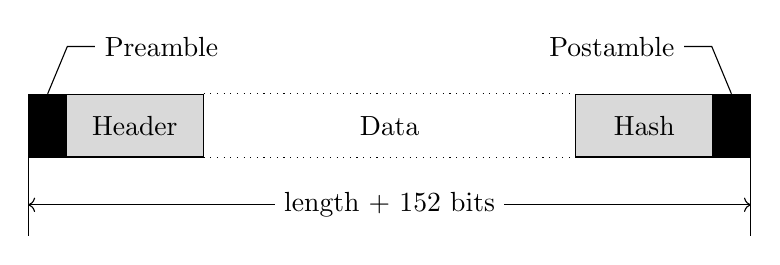
\begin{tikzpicture}[node distance=-\pgflinewidth]

\node[short,fill=black] (preamb) {};
\node[long,right=of preamb,label=center:Header](header){};
\node[verylong,draw=none,fill=none,right=of header,label=center:Data] (data) {};
\node[long,right=of data,label=center:Hash] (hash) {};
\node[short,fill=black,right=of hash] (postamb) {};

\node[above right=0.5cm of preamb] (ppre) {Preamble};
\node[above left=0.5cm of postamb] (ppos) {Postamble};

\draw (ppre.west) -- +(-10pt,0pt) -- (preamb.north);
\draw (ppos.east) -- +(10pt,0pt) -- (postamb.north);
\draw[dotted] (header.north east) -- (hash.north west);
\draw[dotted] (header.south east) -- (hash.south west);
\draw[<->] ( $ (preamb.south west) +(0,-0.6cm) $ ) -- node[fill=white] {length + 152 bits} ( $ (postamb.south east) +(0,-0.6cm) $ );
\draw (preamb.south west) -- +(0,-1cm);
\draw (postamb.south east) -- +(0,-1cm);

\end{tikzpicture}
\caption{Packet structure}
\label{fig:packet}
\end{figure}

Preamble is a predefined 64-bit sequence \textsf{0xa5a5a5a5a5a5a5a5}. Postamble is a bitwise-inverse of the preamble. Header is an 8-bit word containing byte-length of the data section in the packet. The shortest size of the data section is 64 bits, while the largest is 248 bits. The data section is always byte-aligned; i.e. its length is always a multiple of 8 bits.

All the words in the packets are stored in big endian notation. The packets are sent further through the transmitter chain sequentially, without a guard interval.

The binary sequence of the generated packets is brought to a QPSK modulator. Its constellation is represented by Figure \ref{fig:qpsk}.

\begin{figure}[h!]
\centering
\begin{tikzpicture}
\begin{axis}[
	xmin=-1.5,xmax=1.5,
	ymin=-1.5,ymax=1.5,
	axis lines=center,
	xlabel=$\Re e$,
	ylabel=$\Im m$,
	xtick={-1,...,1},
	ytick={-1,...,1},
]
\addplot+ [nodes near coords, only marks, point meta=explicit symbolic]
table[meta=label]{
	x	y	label
	1	1	00
	-1	1	01
	-1	-1	11
	1	-1	10
};
\end{axis}
\end{tikzpicture}
\caption{QPSK modulator constellation}
\label{fig:qpsk}
\end{figure}

The QPSK-modulated symbols are transposed to carrier frequency $f_c = 36 \,\textrm{kHz}$ and transmitted by a hydrophone. Transmitter data-rate is 9.6 kbit/s. At the receiving end, the receiver aboard a submarine is depicted by a block diagram in Figure \ref{fig:task1}.

\begin{figure}[h!]
\centering
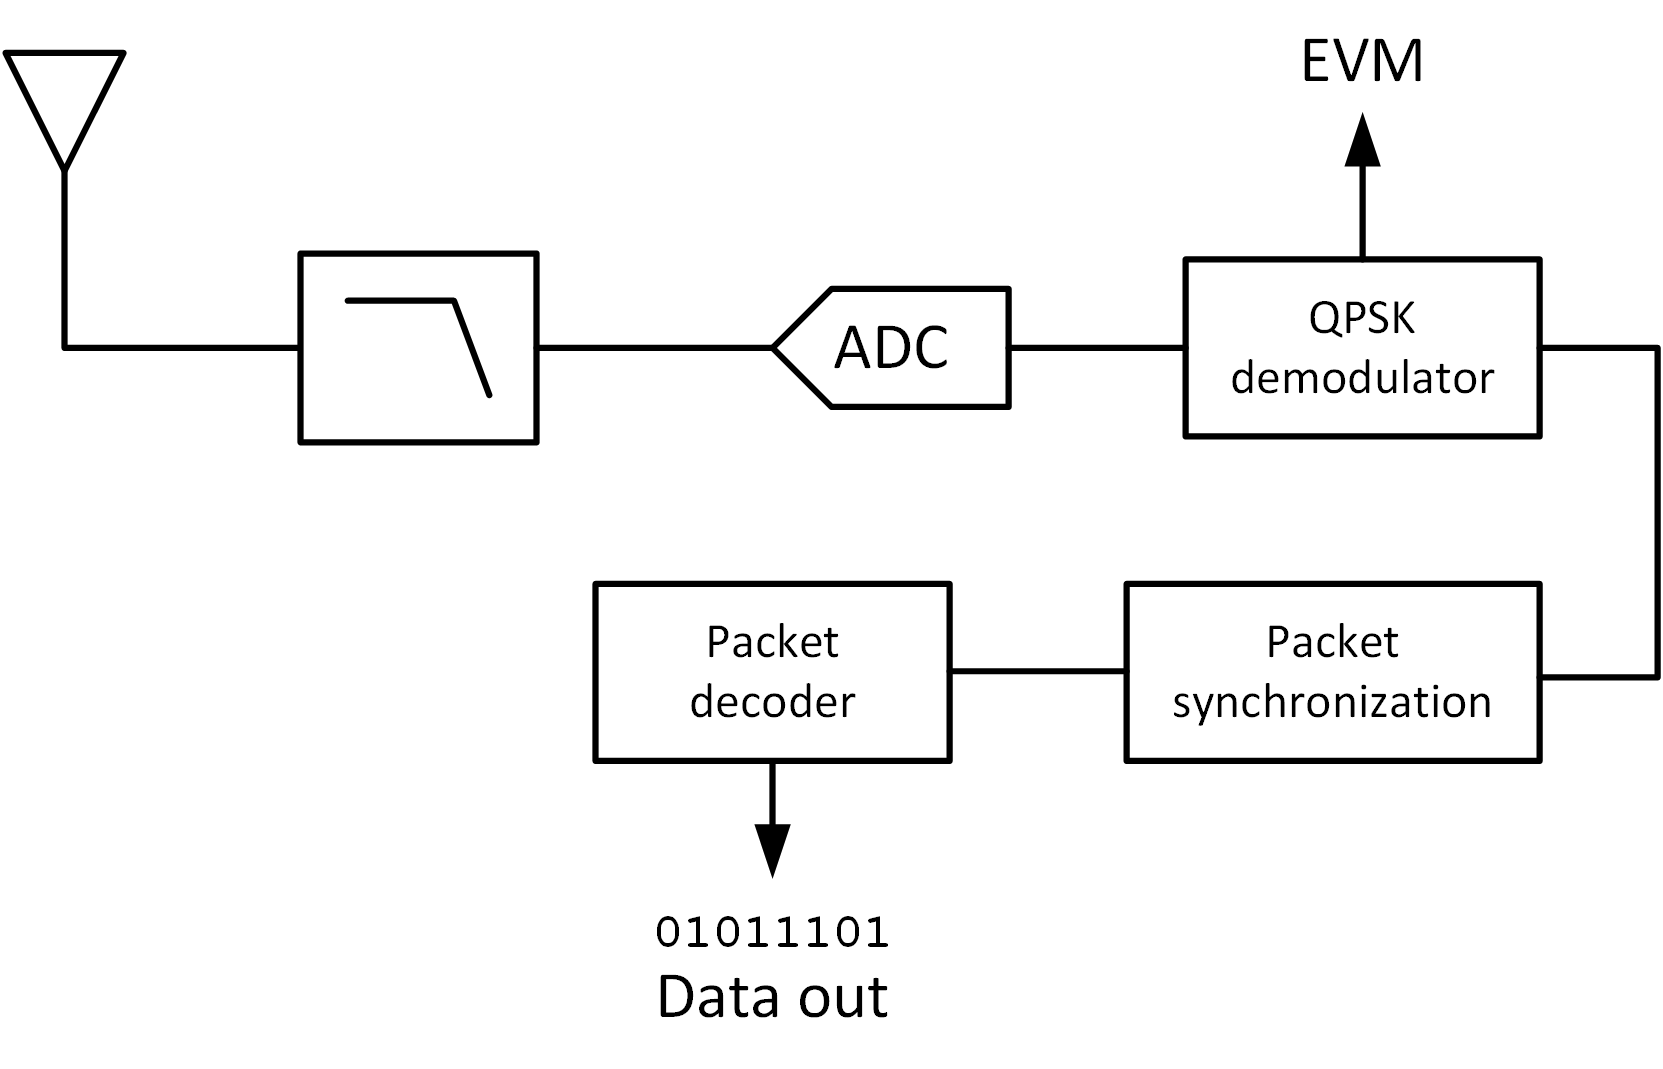
\includegraphics[width=0.9\textwidth]{Images/Task1.png}
\caption{Receiver diagram in Task 1}
\label{fig:task1}
\end{figure}

The ADC of the receiving hydrophone operates at a sampling frequency of 192 kSps. An ideal low-pass filter has a cut-off frequency of 96 kHz.

You are required to implement the digital processing system of the receiver, to demodulate and decode information from the received ultrasonic signal.

\subsubsection{Input data}
The \textsf{single\_carrier.raw} file is given. It contains the digitized signal from the ADC, recorded in 16-bit 2's complement format.

\subsubsection{Implementation}
Your solution is a C or C++ code implementing the receiver's digital processing chain. Your solution consists of two files:
\begin{description}
	\item[radio.c / cpp] Implements all the routines described further in the text.
	\item[main.c / cpp] Loads the input data, calls the routines from \textsf{radio.c / cpp}, and outputs decoded data to stdout in the original format.
\end{description}

Your \textsf{radio.c / cpp} file must implement the following set of functions:
\begin{description}
	\item[complex *frequency\_shift(double *input, double fc, double fs, int N)]
	\,\\ Transposes the signal provided in input from centre frequency \textsf{fc} to baseband. \textsf{N} is the length of the data stream, expressed as a number of double words. \textsf{fs} is the sampling frequency.
	\item[double qpsk\_demodulator(complex symbol, double constellation\_offset, char *decoded\_symbol)]
	\,\\ Decodes a baseband QPSK symbol \textsf{symbol}, and stores its value to an 8-bit word \textsf{decoded\_symbol}. The function outputs the EVM of the symbol.
	\item[char *bitstream\_to\_bytestream(char *bitstream, int length)]
	\,\\ Converts \textsf{length} 8-bits words, as output by the \textsf{bitstream\_to\_bytestream} function, into a bytestream. Parameter \textsf{length} is the length of the bitstream array, while the length of the output array is equal to \textsf{length}/4. A pointer to the beginning of the bytestream is returned.
	\item[void frame\_sync(char **bytestream, int length)]
	\,\\ Moves the pointer \textsf{*bytestream} to the beginning of the first detected frame. \textsf{length} is the length of the bytestream.
	\item[int frame\_decoder(char *bytestream, char **data)]
	\,\\ Decodes the data from a single frame that starts at the pointer \textsf{*bytestream}. The decoded data should be stored to \textsf{*data}. The return value is the length of processed data (frame length).
\end{description}

You are provided with some helper files:
\begin{description}
	\item[radio.h]
	\item[api.h]
	\,\\ An API containing some types, functions and constants you may find useful.
	\item[api.c]
	\,\\ The compiled API described in \textsf{api.h}.
\end{description}


\subsubsection{Evaluation}

You have access to an evaluation server to which you can upload your source files.
The server will execute your code and verify the functionlity of each function implemented in your \textsf{radio.c / cpp} file,
and the functionality of the entire processing chain, by executing the program in \textsf{main.c / cpp}.
The server functionality will further be described in a document that you will receive at the start of the competition day.

\subsection{Task 2}

Along the submarine's trajectory information, the habitat and the submarine exchange location data on debris scattered around the sea. This data is transmitted in a separate data stream from the trajectory coordinates, and it has the same triplet format as the data from Task 1. Also, the data is packaged in the same manner as in Task 1. The resulting bitstream is then spread into 4 QPSK subcarriers, as depicted in Figure \ref{fig:spread}.
\begin{figure}[h!]
	\centering
	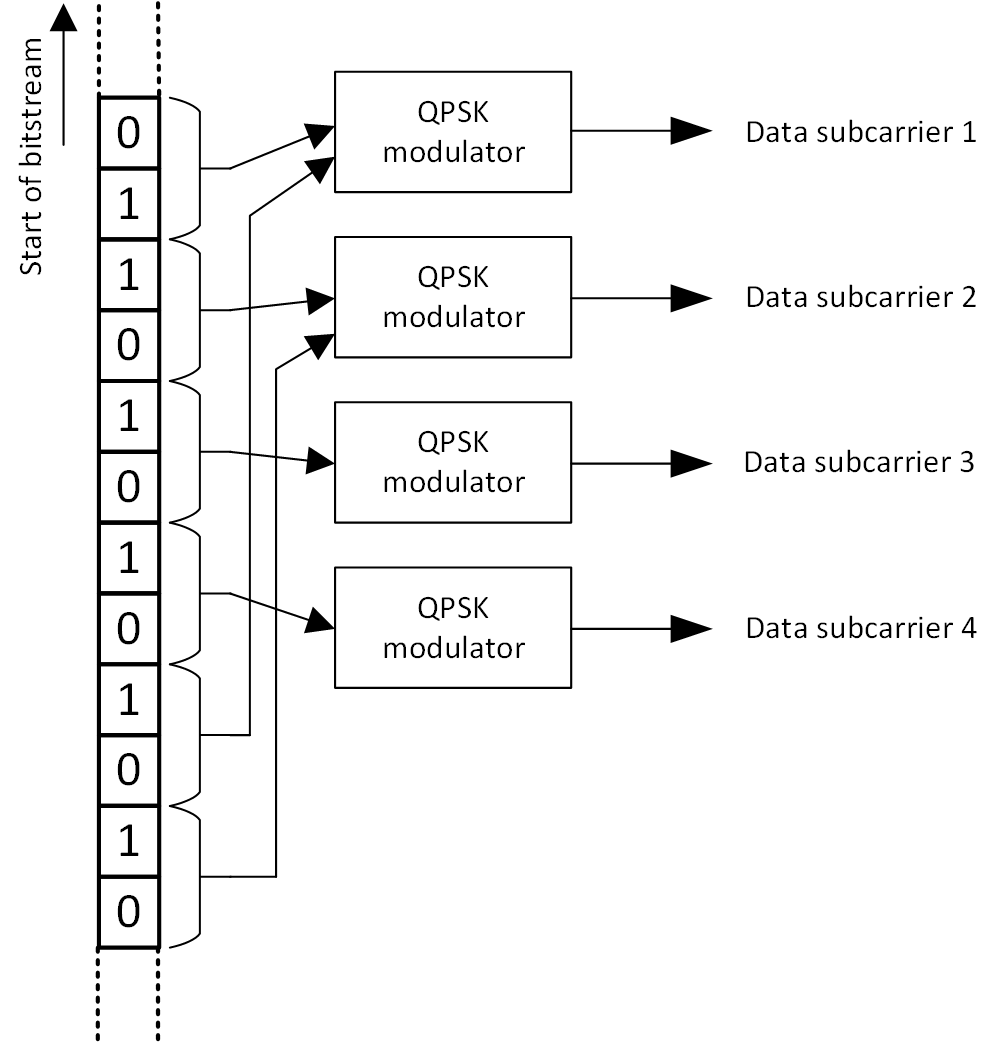
\includegraphics[width=0.7\textwidth]{Images/spread.png}
	\caption{Bitstream spreading mechanism}
	\label{fig:spread}
\end{figure}

The obtained QPSK carriers are multiplexed into OFDM that consists of a total of 9 subcarriers. These are organized as depicted by DFT spectrum in Figure \ref{fig:dft}.
\begin{figure}[h!]
	\centering
	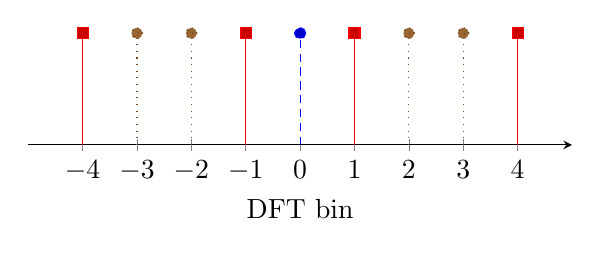
\begin{tikzpicture}
	\begin{axis}[
		width=0.7\textwidth,
		height=3cm,
		axis x line=bottom,
		axis y line=none,
		xlabel=DFT bin,
		ymin=0,ymax=1,
		xmin=-5,xmax=5,
		xtick={-4,...,4}
	]
	% Osnovni podatak
	\addplot+ [ycomb, style={densely dashed}] plot coordinates {
		(0,1)
	};
	% Piloti
	\addplot+ [ycomb, style={solid}] plot coordinates {
		(-4,1) (-1,1) (1,1) (4,1)
	};
	% Ostali nosioci
	\addplot+ [ycomb, style={dotted}] plot coordinates {
		(-3,1) (-2,1)
		(2,1) (3,1)
	};
	\end{axis}
	\end{tikzpicture}
	\caption{OFDM carrier DFT spectrum}
	\label{fig:dft}
\end{figure}

Subcarrier spacing is $\varDelta f = 1500 \,\textrm{Hz}$. The graph in Figure \ref{fig:dft} is centred to frequency $f_c = 36 \,\textrm{kHz}$, corresponding to the central frequency of the OFDM carrier. The subcarrier at bin 0, depicted by a dashed line, contains trajectory coordinate stream from Task 1. Subcarriers depicted by dotted lines contain the data stream added for this task. Subcarriers depicted by a solid line are pilots. OFDM symbols have no cyclic prefix.

The receiver code from Task 1 has to be modified to work with an OFDM carrier, and decode the additional data stream. Block diagram of the receiver is presented in Figure \ref{fig:task2}.

\begin{figure}[h!]
\centering
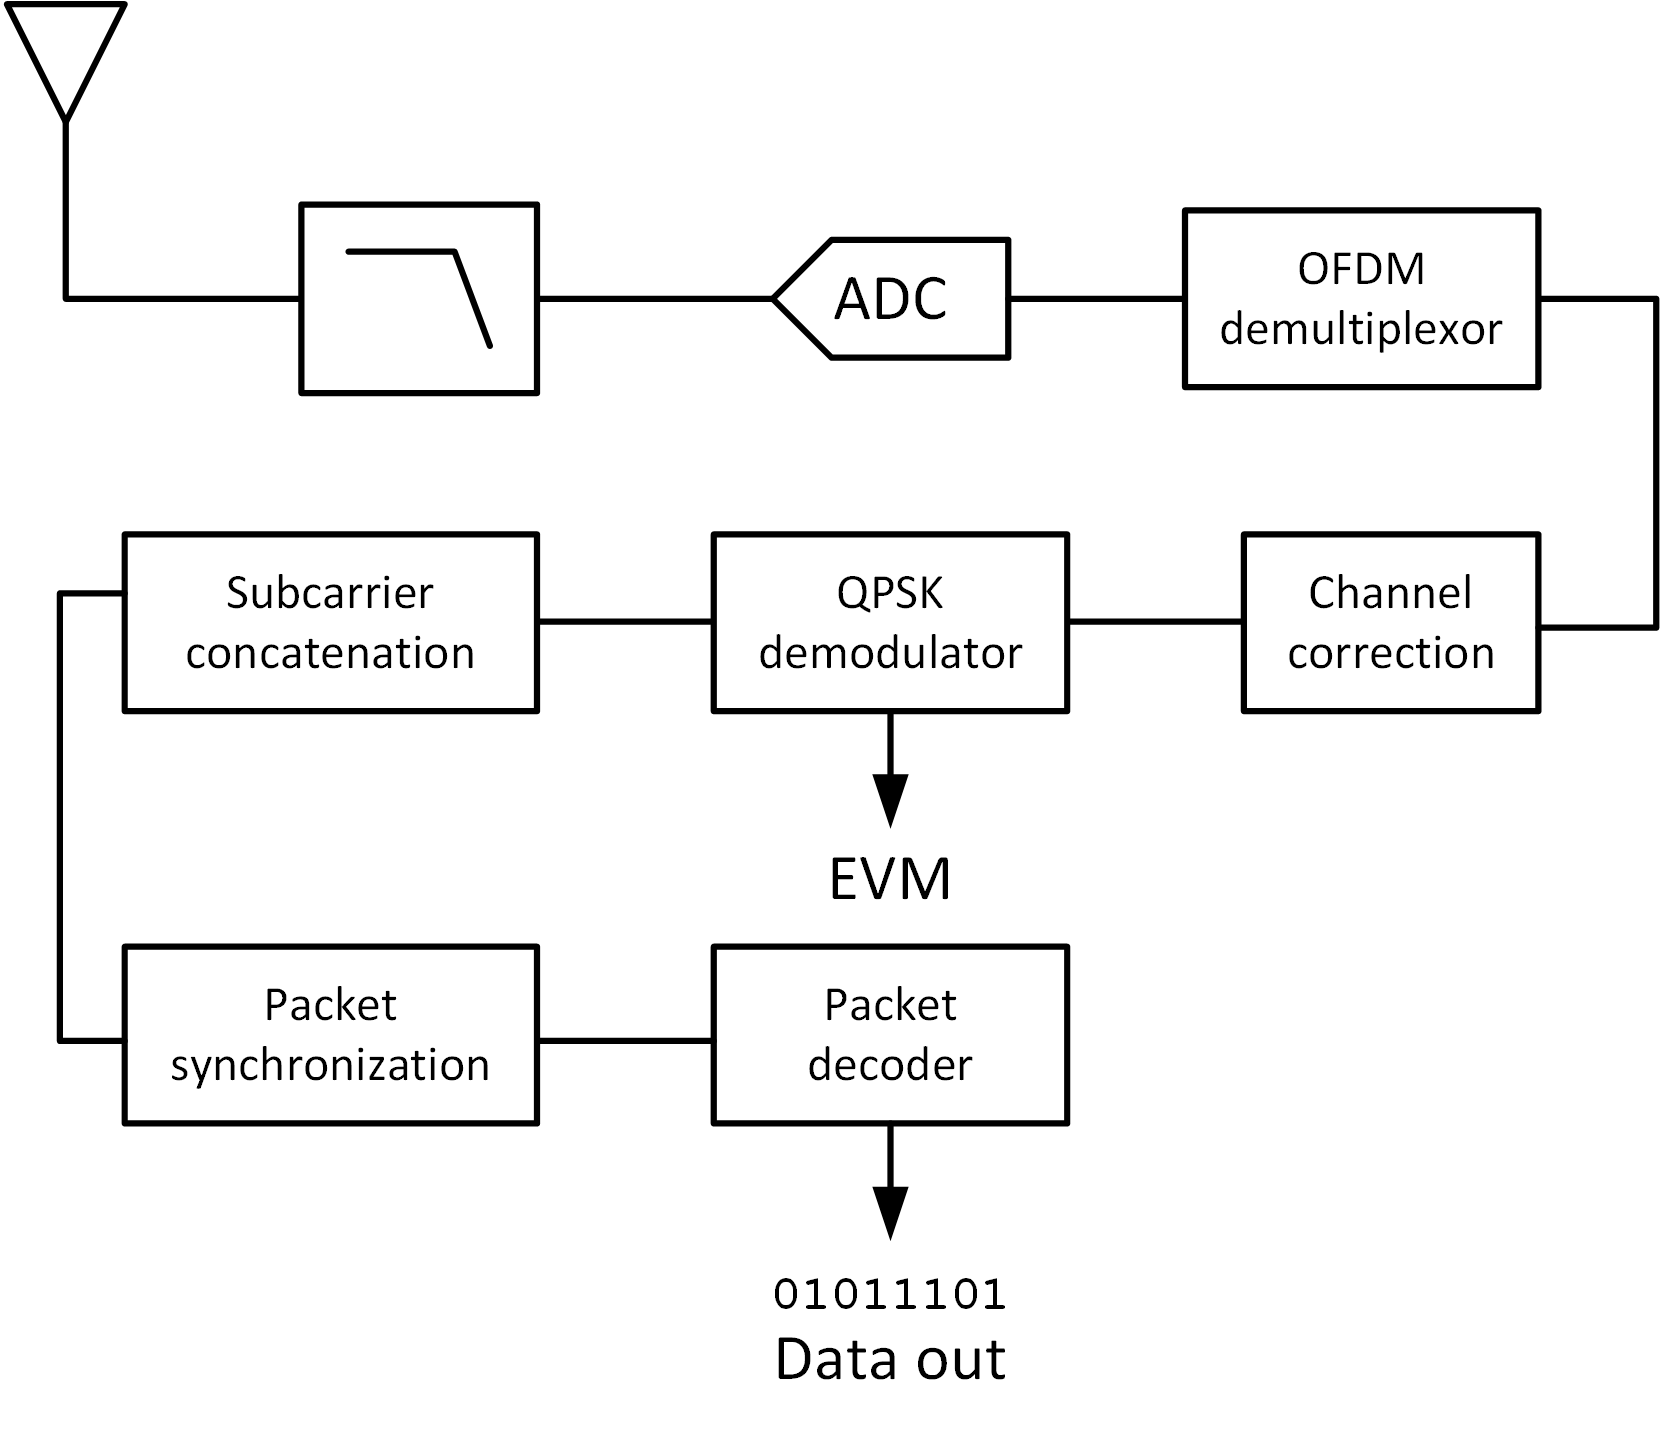
\includegraphics[width=0.9\textwidth]{Images/Task2.png}
\caption{Receiver diagram in Task 2}
\label{fig:task2}
\end{figure}

\subsubsection{Input data}
The \textsf{ofdm\_carrier.raw} file is given. It contains the digitized signal from the ADC, recorded in 16-bit 2's complement format.

\subsubsection{Implementation}
You should update your \textsf{radio.c / cpp} and \textsf{main.c / cpp} to implement the new features required for Task 2. Your \textsf{radio.c / cpp} file should implement the following additional functions:
\begin{description}
	\item[double *ofdm\_demodulator(complex *spectrum, int *carrier\_idx, int carrier\_no, char **data)]
	\,\\ Takes the spectrum of a \underline{single OFDM symbol} from \textsf{*spectrum}, and demultiplexes the subcarriers containing the \underline{additional data stream}. The demodulated QPSK symbols from these subcarriers are stored in a bitstream array that starts at \textsf{*data}. Demodulated QPSK symbols from each subcarrier are stored in their own \textsf{char}s, to be used as input to the \textsf{bitstream\_to\_bytestream} function. The input signal is in baseband in the original sample rate. \textsf{carrier\_idx} is a list of DFT bins that contain the additional data stream. \textsf{carrier\_no} is the length of \textsf{carrier\_idx} array.
\end{description}

\subsubsection{Evaluation}

The same evaluation server as that used in task 1 will serve to verify the functionality of your OFDM-capable receiver.

\subsection{Task 3}
An algorithm for calculating the CRC-16 hash of an input stream should be added to solutions for both tasks. CRC-16 verification should first be implemented as a separate function, and then integrated into the receiver chain. The modification is presented in Figure \ref{fig:task3}.

\begin{figure}[h!]
\centering
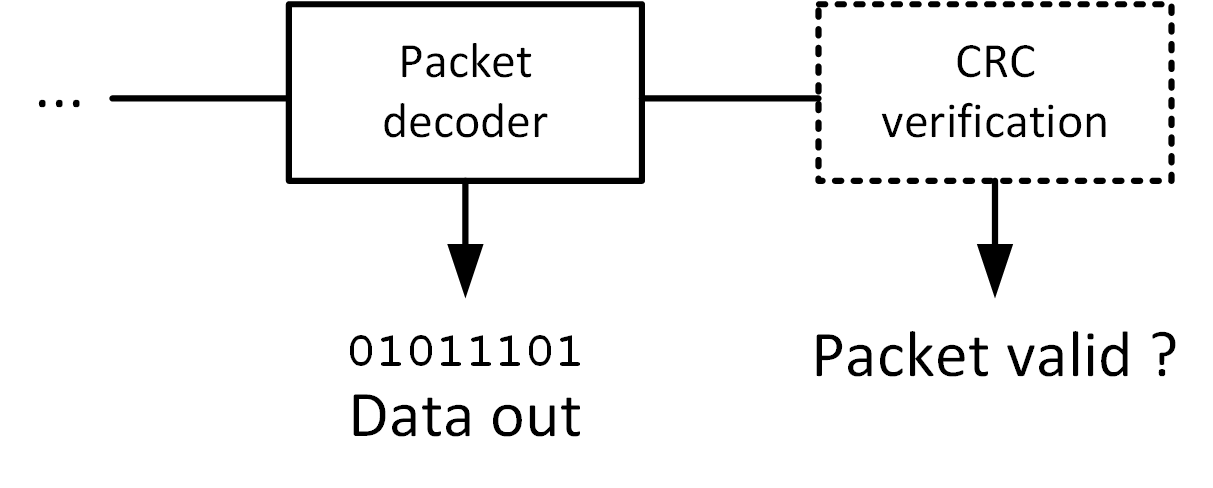
\includegraphics[width=0.7\textwidth]{Images/Task3.png}
\caption{CRC check in receivers}
\label{fig:task3}
\end{figure}

The CRC-16 hash in data frames is calculated using the CRC-CCITT algorithm, with an initial register state \textsf{0xffff}.

\subsubsection{Implementation}
Your \textsf{radio.c / cpp} code must implement the following additional functions:
\begin{description}
	\item[char crc16\_check(char* bitstream, int length)]
	\,\\ Returns CRC-16 hash of the given \textsf{bitstream}, of length \textsf{length}.
	\item[int frame\_decoder\_valid(char* bytestream, char** data, bool *valid)]
	\,\\ Decodes the data from a single frame that starts at the pointer \textsf{*bytestream}. The decoded data should be stored to \textsf{*data}. The output flag \textsf{*valid} denotes if the decoded frame has a valid CRC-16 checksum. The return value is the length of processed data (frame length).
\end{description}

\subsubsection{Evaluation}

The same evaluation server as that used in tasks 1 and 2 will serve to verify the functionality of your error-detection algorithm.

\subsection{Documentation}

Provide documentation that describes your solution for the receiving chain. Back your implementation by describing the mathematical background of your processing chain. Document the datasets you used to evaluate your solution.

The documentation will not be graded, but it can help mentors in understanding your approach and validating the theory behind your solution.
	
\newpage
\section{Synchronous machine design}

\subsection{Introduction}

Your submarine needs electric power to drive the main propeller shaft and to operate all the equipment on board. The main supply of the electric power on your submarine is a synchronous generator. The generator rotor is fitted on the same shaft as the steam turbine. The generator converts the mechanical power from the steam turbine into electrical energy which is supplied to each load on the submarine. Generators are typically purchased based on the requirements of a specific application. In this task you will be designing a three-phase synchronous generator for your submarine. Nominal values of the synchronous generator are given as: 
\begin{table}[h!]
    \hyphenpenalty 10000
    \caption{Nominal values of the generator}
    \label{tab:nominalValues}
    \begin{tabularx}{\textwidth}{|Y|Y|Y|Y|} \hline
    \textbf{No. of Phases} & 3 & \textbf{Frequency} & 50 Hz \\ \hline \textbf{Voltage} & 400 V, {\Large $\wye$} & \textbf{Speed} & 3000 rpm \\ \hline
    \textbf{Power rating} & 70 kVA & \textbf{Power factor} & 80 \% \\ \hline
    \end{tabularx}
\end{table}

\subsection{Calculation of the machine parameters}
Synchronous generator design is not a simple task and to make it easier for you only a limited  number of parameters needs to be determined. 
\\The main dimensions of the generator that you need to calculate are:
\begin{itemize}
    \item the stator bore diameter,
    \item the rotor diameter,
%    \item the air gap length.
\end{itemize}
All of the machine main dimensions must be calculated in meters.
\\Next, you have to determine:
\begin{itemize}
    \item the number of conductors in the stator slots (round to the first higher integer),
    \item the number of field winding turns (integer).
\end{itemize} 
Lastly, the design of the generator is finished with the calculation of the synchronous reactance in p.u. 
\\Generators used in applications with steam turbines (high-speed applications) are ones with a cylindrical (round) rotor. The rotor body of the generator is typically a solid piece of steel for reasons of strength, given the high rotational speeds to which the rotor is subjected. The rotor diameter is sized to operate at near the stress limit of the steel alloy. The maximum allowable peripheral speed of the generator is $80\ \mathrm{m/s}$ which means the machine must be capable of sustaining 70 \% overspeed. 
\\Windings located on the rotor of the generator are called field (excitation) windings. Field windings are supplied with direct current. The external source used to provide DC current is commonly referred to as an exciter. At the no-load condition, the exciter supplies field windings with DC current equal to $28\ \mathrm{A}$ which is required to create a field current linkage of $1904\ \mathrm{A}$. In order to describe the magnetic circuit of the machine and the required field current linkage, Ampere's law may be used. The current linkage produces magnetic flux density sinusoidally distributed along the pole. During half of the period $T$ the flux density wave travels one stator pole pitch. The maximum value of the magnetic flux density in the air gap is 0,8 T and the length of the air gap is constant. Iron's magnetic permeability can be assumed to be infinite in comparison with the magnetic permeability of air. 
Stator windings or armature windings are full-pitch one-layer windings embedded in 36 slots. Stator length is $0.5\ \mathrm{m}$. A synchronous generator can be represented by a simple equivalent circuit as shown in figure \ref{fig:01}. Phase voltage measured on the output terminals of the generator is lower than the induced phase voltage due to the voltage drop on the stator impedance. The synchronous reactance prevails in the stator impedance which means that the stator resistance can be neglected when calculating the synchronous reactance. In nominal conditions (nominal voltage, power factor and load) the angle between the terminal voltage and the induced voltage is equal to $25.07^{\circ}$.
\begin{figure}[!htb]
			\centering
			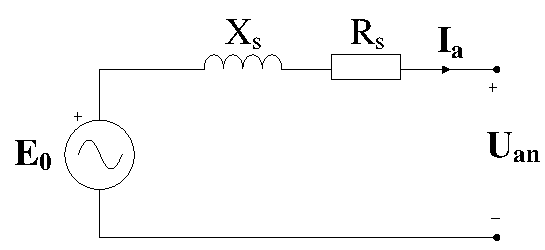
\includegraphics{Images/EquivalentCircuit.pdf}
			\caption{Synchronous machine equivalent circuit}
			\label{fig:01}
\end{figure}
In order to determine the characteristics of the synchronous generator standardized tests must be carried out. The simplest method by which this is achieved are the open-circuit and the short-circuit tests. Typical open-circuit and short-circuit curves are shown in figure \ref{fig:02}. During the open-circuit the field winding is supplied with the nominal field current $I_{fn}$ and the phase voltage measured on the generator terminals is equal to $680.235\ \mathrm{V}$. In case when the field current is equal to $I_{f0} = 28 \ \mathrm{A}$, the voltage measured at the generator terminals will be equal to the nominal voltage. During the short-circuit test when the field winding current equals to $I_{f0}$ the measured stator current will be $64.762\ \mathrm{A}$. 
\\The per-unit system is widely used within the analysis of electrical machines. Per-unit values are obtained by dividing each parameter by a base value. For this task the base values are defined with:
\begin{itemize}
    \item peak value of the rated stator phase voltage,
    \item rated apparent power,
    \item rated angular frequency,
    \item peak value of the rated stator phase current.
\end{itemize}


\begin{figure}[!htb]
			\centering
			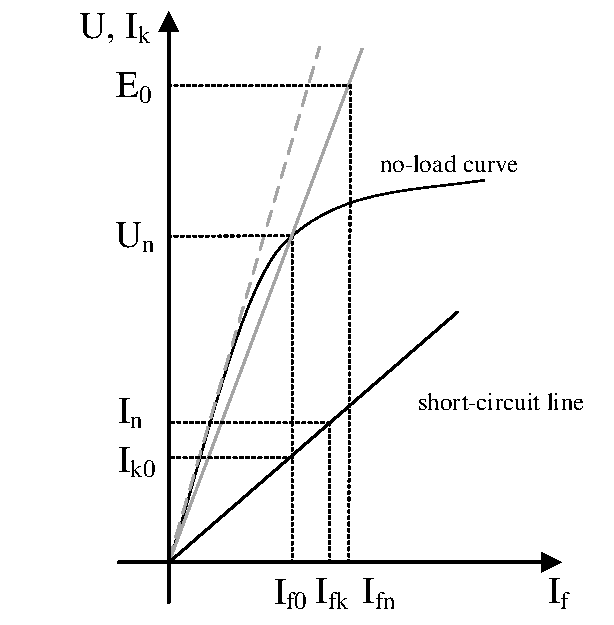
\includegraphics[scale=0.5]{Images/NoLoadCurveShortCircuit.pdf}
			\caption{Open-circuit and short-circuit curves}
			\label{fig:02}
\end{figure}
\newpage
\subsection{Solution format and grading scheme}
Your solution must be submitted as a .csv format document with only 2 rows. File name must be 
\texttt{machineParameters.csv}. The first row must consist of the required parameter names and the second row of numerical values that you calculated for each parameter. Column names must be marked as follows (columns should be in exactly this order):
\begin{itemize}
    \item stator bore diameter \textbf{Ds},
    \item rotor diameter \textbf{Dr},
    \item air gap length \textbf{delta},
    \item number of conductors in the stator slots \textbf{z},
    \item number of field winding turns \textbf{Nf},
    \item synchronous reactance in p.u \textbf{Xd}.
\end{itemize}
This task is graded up to 20 points. 3 points are given for  each correctly calculated parameter and 2 points are given for the documentation. The documentation is submitted at the end of the day. The documentation must include your calculations along with some short comments explaining the equations. You can choose the format in which the documentation will be submitted (.c script, .m script, hand written equations).
	
\end{document}
